\section{Arquitetura}

    Antes de implementar qualquer estrutura de dados propriamente dita, é necessário estabelecer e definir uma arquitetura que possibilite as funcionalidades básicas de qualquer rede \textit{peer-to-peer}. Felizmente essa arquitetura já foi definida há muitos anos, e, portanto, mais vale percorrer um caminho previamente conhecido, do que tentar inventar algo novo e correr o risco de não funcionar devidamente.

    \begin{figure}[hb!]
        \centering
        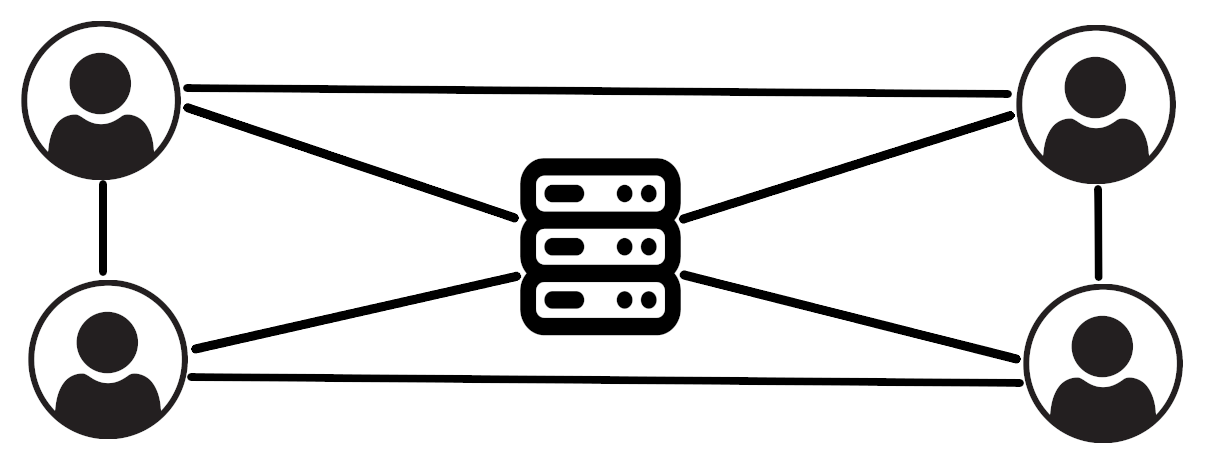
\includegraphics[width=0.7\textwidth]{Imagens/Estruturas/peer-to-peer.png}
        \caption{Arquitetura simplificada de uma rede \textit{peer-to-peer}}
    \end{figure}

    Tal como mandam as regras, no centro da rede encontra-se o \textit{tracker}, cuja função é única e exclusivamente anunciar aos clientes onde se encontram os ficheiros que estes pretendem adquirir, consequentemente concluímos que este elemento não contribuí diretamente para a transferência de quaisquer conteúdos que os clientes possuam.

    Já em relação ao cliente, a situação torna-se um pouco mais complexa, pois após receber as informações do \textit{tracker} e iniciar a sua transferência de dados com os outros clientes, o mesmo deve permitir que os seus próprios ficheiros continuem a ser partilhados, o que requer um comportamento \textit{multithreading} por parte deste agente.

    \subsection{Identificação de Blocos}

        Qualquer serviço descentralizado tem como objetivo distribuir a carga de trabalho pelos diversos agentes, e tendo em conta que neste caso um agente corresponde a um cliente, é necessário garantir que os ficheiros não são tratados como blocos atómicos, visto que isso impossibilita a receção de dados a partir de vários clientes.

    
        \begin{figure}[hb!]
            \centering
            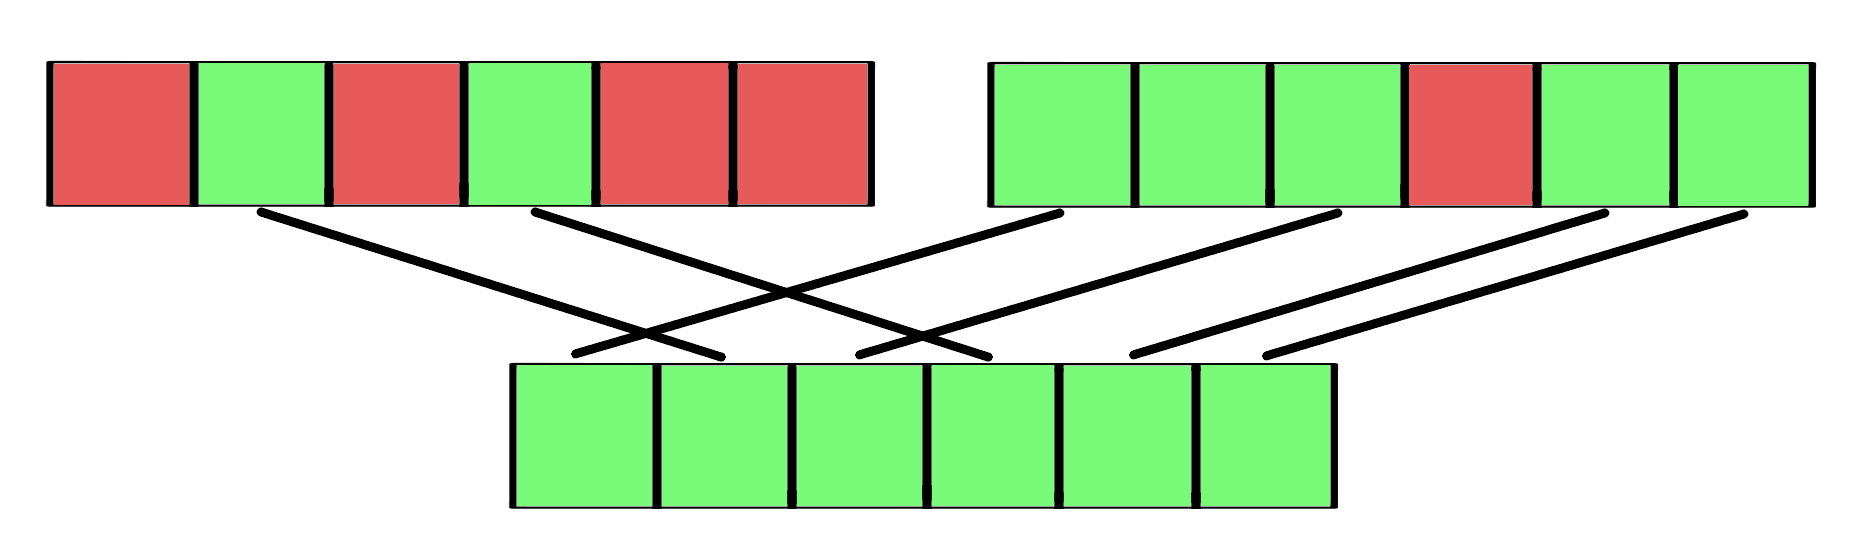
\includegraphics[width=0.65\textwidth]{Imagens/Blocos/blocos.png}
            \caption{Divisão de um ficheiro em blocos}
        \end{figure}
        \vspace{-10pt}

        Se pensarmos que um ficheiro é na realidade um conjunto de blocos de tamanho fixo (apenas o último é variável), cada cliente pode enviar aquilo que possui, e assim estão todos a contribuir para que um único ficheiro seja transmitido pela rede. Além disso, esta estratégia evidencia um efeito secundário bastante interessante, no qual um cliente pode obter um ficheiro sem que nenhum dos restantes o tenha na totalidade.

        A ideia dos blocos é muito poderosa, mas levanta uma série de outras questões.
        
        \begin{itemize}
            
            \item De que forma um cliente sabe que possui o bloco \textit{A} em vez do \textit{B}?  

            \item Como é possível um cliente descobrir a posição relativa dos seus blocos?
        \end{itemize}

        A resposta a estas perguntas é muito simples, \textit{hash}! Se cada bloco tiver um código associado, muito facilmente concluímos a igualdade entre dados, e tendo em conta que o \textit{tracker} fica a conhecer todos os códigos no momento em que um ficheiro é anunciado, rapidamente podemos deduzir as posições dos blocos que outros clientes eventualmente possuam.

        A criação de um código como resultado de uma função de \textit{hash} é bastante comum nos dias de hoje, contudo, neste caso em particular, basta uma colisão para arruinar a identificação de um ficheiro na estrutura de dados do \textit{tracker}.

        \begin{figure}[hb!]
            \centering
            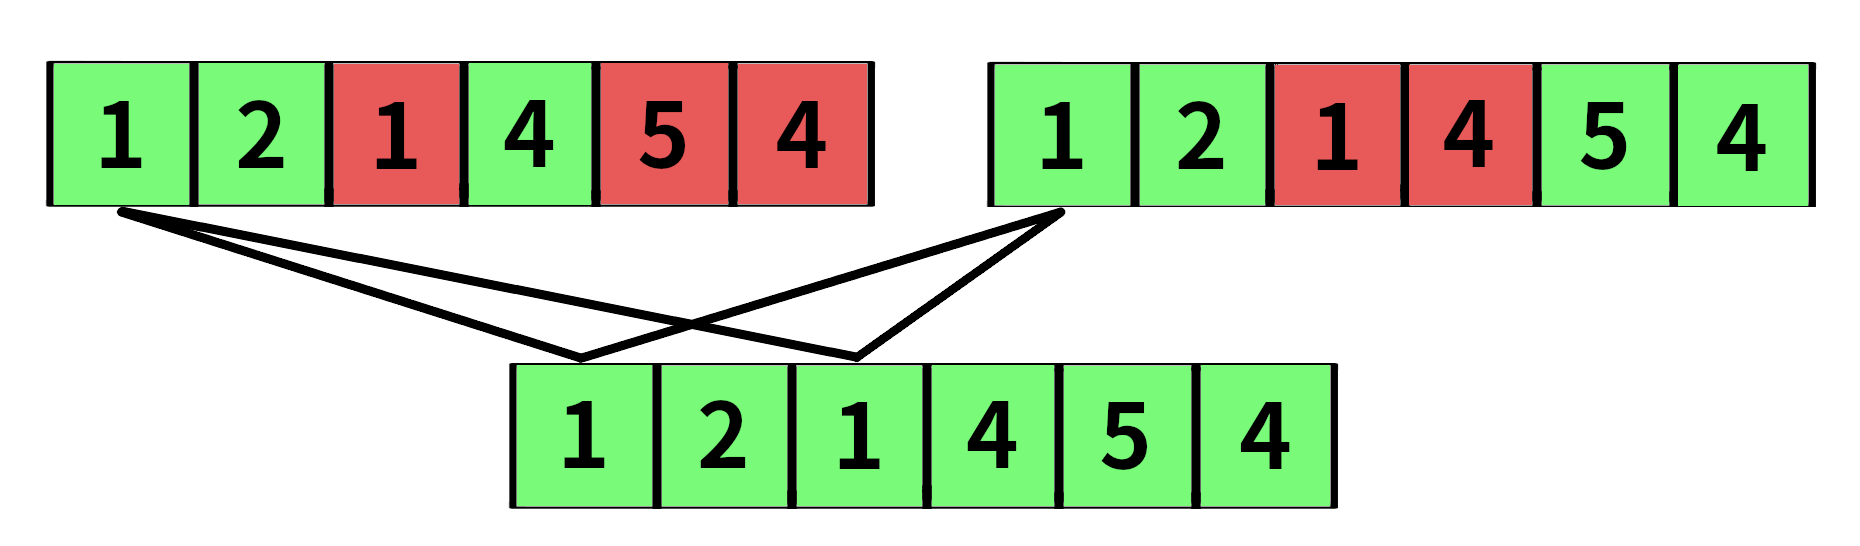
\includegraphics[width=0.65\textwidth]{Imagens/Blocos/colisao de blocos.png}
            \caption{Colisão de blocos}
        \end{figure}
        \vspace{-10pt}

        Nesta situação, o primeiro e terceiro bloco do ficheiro original possuem o mesmo código de \textit{hash}, consequentemente nenhum dos restantes clientes sabe a posição dos seus blocos, o que por sua vez origina grandes problemas no momento de realizar a transferência e fazer o \textit{reassembly}.

        Não existe uma solução perfeita capaz de evitar colisões, o melhor que se pode fazer é minimizá-las, em particular através da utilização de funções de \textit{hash} bastante poderosas.

        Após analisarmos o comportamento do \textit{BitTorrent} face a esta situação, verificámos que o mesmo aplicava uma função de dispersão criptográfica (\textit{SHA-1}) a blocos de tamanho entre 32 \textit{KB} e 16 \textit{MB}, pelo que decidimos seguir a mesma estratégia, todavia com blocos de 2048 \textit{bytes}.

        É possível pensar que 2048 \textit{bytes} é insuficiente para o problema em questão, contudo julgamos que muito dificilmente existem blocos com o mesmo código de \textit{hash}. Até porque ao criarmos um ficheiro de 1 \textit{GB}, verificámos que o \textit{tracker} identificou o número expectável de blocos (a contagem começa em zero).

        \[
            \text{\textit{Número de blocos}} 
                = \dfrac
                    {10^{9}}
                    {2048}
                = 488281,25
                \simeq 488282 ~\text{\textit{blocos}}
        \]

        \begin{figure}[hb!]
            \centering
            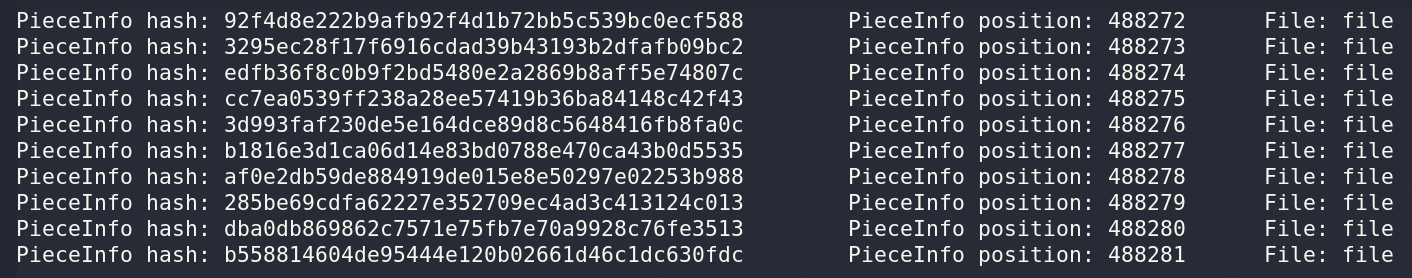
\includegraphics[width=0.8\textwidth]{Imagens/Blocos/teste de colisoes.png}
            \caption{Teste de colisão de blocos}
        \end{figure}